\chapter{Structures and Materials}
\label{ch:Structures_and_Materials}
In this chapter, the material selection for the most crucial aircraft components will be performed.
Additionally, the wing structure shall be designed taking the limit load factors into account.
Lastly, based on the wing design, the load applied on the hing, as well as the folding mechanism, shall be sized.
Finally, the landing gear configuration shall be discussed.
\section{Materials selection}
\label{sec:matselection}
Materials are an essential part of aircraft structural design.
It is the different material properties that allow for the sizing of structural components.
Different materials are suitable for different parts based on their properties and loads to be carried. \Cref{tab:matproperties} introduces the characteristics of the materials considered in the design of the eVTOL. Density ($\rho$), Young's Modulus ($E$), ultimate tensile ($\sigma_{\text{t,ult}}$), compressive ($\sigma_{\text{c,ult}}$), and shear ($\tau_{\text{ult}}$) stresses, as well as the poisson ratio ($\nu$) are indicated. 

\begin{table}[H]
    \caption{Structural materials mechanical properties}
    \label{tab:matproperties}
    \centering
        \begin{tabular}{l|SSSSSSS}
            \toprule
            & \textbf{$\rho$ [\unit{g/cm^3}]} & \textbf{$E$ [\unit{GPa}]} & \textbf{$G$ [\unit{GPa}]} & \textbf{$\sigma_{\text{t,ult}}$ [\unit{MPa}]} & \textbf{$\sigma_{\text{c,ult}}$ [\unit{MPa}]} & \textbf{$\tau_{\text{ult}}$ [\unit{MPa}]} & \textbf{$\nu$ [\unit{-}]} \\ \midrule
            \textbf{Al 7040-T7451} \cite{Al7040} & 2.82 & 66 & 24.5 & 438 & 351 & 303 & 0.33 \\
            \textbf{CF Fabric} \cite{CFRP} & 1.60 & 70 & 5.0 & 600 & 570 & 90 & 0.10 \\ \bottomrule
        \end{tabular}
\end{table}

Before a structural analysis is performed, materials can already be selected based on the functions to be fulfilled by the different parts, the types of loads expected, and the literature.
General structural design criteria useful for material selection - like the one shown by P. Jerome \cite{jerome2001composite} - have thus been revised for the \textit{Swing} and are shown in \Cref{fig:matdesigncriteria}.


\begin{figure}[H]
    \centering
    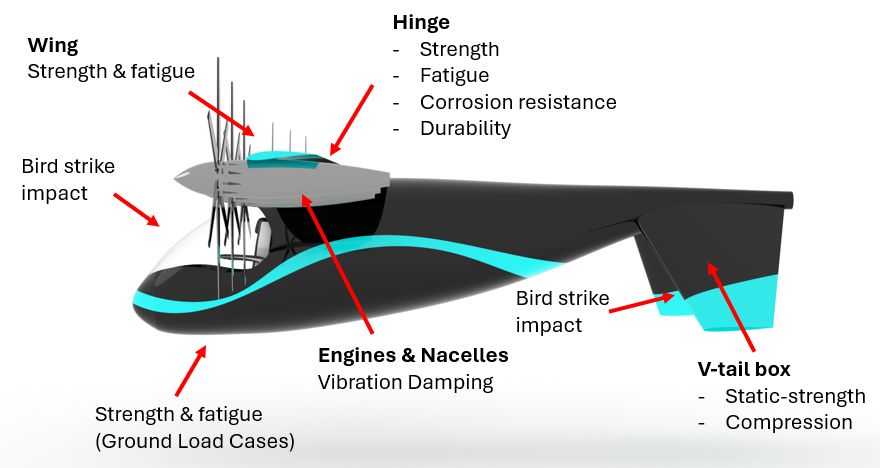
\includegraphics[width=0.8\linewidth]{figures//Structures/MaterialsCriteria.png}
    \caption{Structural design criteria}
    \label{fig:matdesigncriteria}
\end{figure}
 

The use of composites in aircraft has increased drastically in the past decades.
Take, for example, the Airbus A380: a lot of new Carbon-Fibre Reinforced Polymer (CFRP) parts have been added and tested, including the main and tail wing box \cite{jerome2001composite}.
This demonstrates the ability of these components to withstand more important loads.
The use of CFRP comes with incredible weight advantages, leading to 20\% to 50\% savings \cite{AircraftComposites}.
In addition, the availability of bigger autoclaves compared to the past allows for the manufacturing of bigger composite parts, facilitating the assembly process.
These types of composites, however, do come with disadvantages like higher costs and non-visible material damage. \Cref{fig:matcost}~\cite{jerome2001composite} showcases how manufacturing and material costs of composites compare to metals, with a comprehensive cost of composite parts around 40\% higher than that of metals \cite{pinto2017economic}. The higher costs of metal in terms of aircraft manufacturing shown in the figure is due to the higher number of components that need to be assembled due to the limited size of metal parts. 
More extensive considerations on the cost are made in the cost analysis in \Cref{ch:Financial_Analysis}.
It can be said, however, that the increase in cost remains within the production cost constraints initially established.
Last but not least, the sustainability of these materials will be evaluated in \Cref{ch:Sustainability_Approach}.

\begin{figure}[htpb]
    \centering
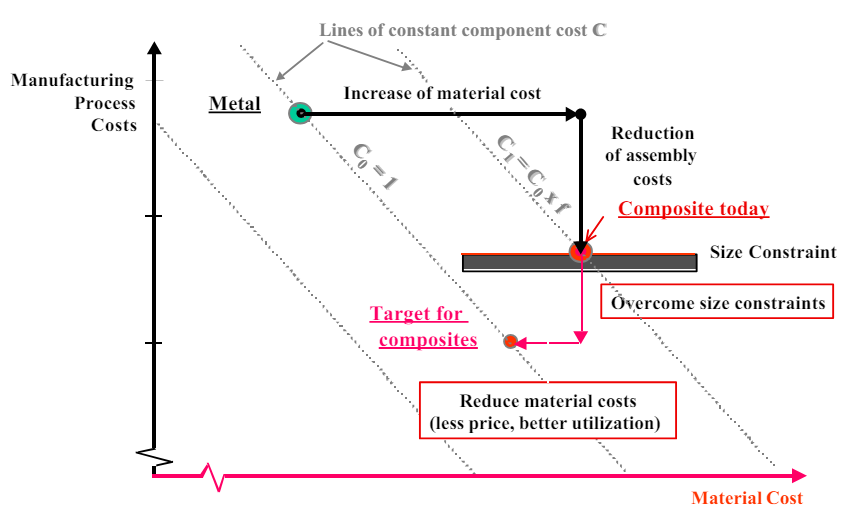
\includegraphics[width=0.8\linewidth]{MaterialsCost.png}
    \caption{Status and targets for cost of composite structures \cite{jerome2001composite}.}
    \label{fig:matcost}
\end{figure}

A preliminary material selection is carried out.
This might be revised in later stages in case the structural analysis uncovers deficiencies in the design.
CFRP is expected to be used on most of the aircraft structure given its weight advantages.
Compared to general aviation aircraft, fatigue loads acting on the fuselage are not considered critical given the absence of fuselage pressurisation.
This allows the use of materials like CFRP, for which crack growth is of bigger concern compared to, for instance, aluminium alloys.
Taking inspiration from aircraft like the A380, the wing box, as well as the ribs, are constructed with CFRP, with the rest of the internal structure in aluminium. The entirety of the tail, instead, is expected to be manufactured with CFRP.

Fiber Metal Laminates (FMLs) are also considered.
In particular,
Glass Reinforced laminate (Glare) is preferred over CARALL (carbon-reinforced aluminium laminate) and ARALL
(aramid-reinforced aluminium laminate)
due to its more widespread use in the aerospace industry as well as its low weight.
It is its lightweight properties that make it not suitable for structural elements.
It will instead be used for leading edges and the parts of the fuselage most exposed to impact.
This is thanks to the excellent tolerance to impact and damage of this composite, as found by Annamalai et al. \cite{ANNAMALAI20211371}.


\subsection*{Fuselage Soundproofing}
\label{subsec:fuselagesoundproofing}
In order to meet the 60dBA of requirement CO-3-STK07-2, the fuselage needs to be soundproof enough to be able to cut the near-field noise of 80dBA (at a 7ft distance, \Cref{fig:noisePlots}) down to 60dBA (decrease of 20dBA).
State-of-the-art soundproofing materials and techniques can ensure reductions in noise levels of up to 55dBA, putting the \textit{Swing} in an ideal spot with respect to a low cabin noise.
For instance, covering the inside of the fuselage in a single layer of 1/8 inch Mass-Loaded Vinyl (MLV) already provides a reduction of about 26 dBA.
This improvement could, however, be hindered by the presence of a large frontal window, which is likely to be a weak point in soundproofing.
Double-glazing windows, consisting of two layers of glass with an air gap in between, would be needed to ensure the 26dBA reduction is kept inside the cabin at all times.
While MLV is a very affordable, easily available OTS material, double glazing windows might turn out to be costly (even in the order of \$10,000 for custom, irregularly-shaped windows); this has to be accounted for in \Cref{sec:Cost_Breakdown_Structure}.

 
\section{$V$-$n$ Diagram}
\label{sec:V-n_Diagram}

Using a load diagram, the maximum load factor can be determined.
The $V$-$n$ diagram is created based on the method described by Roskam~\cite{Roskam_Part_2}.
The load diagram can be found in \Cref{fig:struc:Load_diagram}; from the load diagram, it can be seen that the manoeuvre speed is higher than the cruise speed.
This is because the manoeuvre speed is calculated based on empirical formulas in contrast, the cruise speed is defined based on requirement \textbf{Te-2-STK07-3-2}.
Additionally, it can be seen that the maximum load factor is caused by the manoeuvre loading.

\begin{figure}[h]
    \centering
    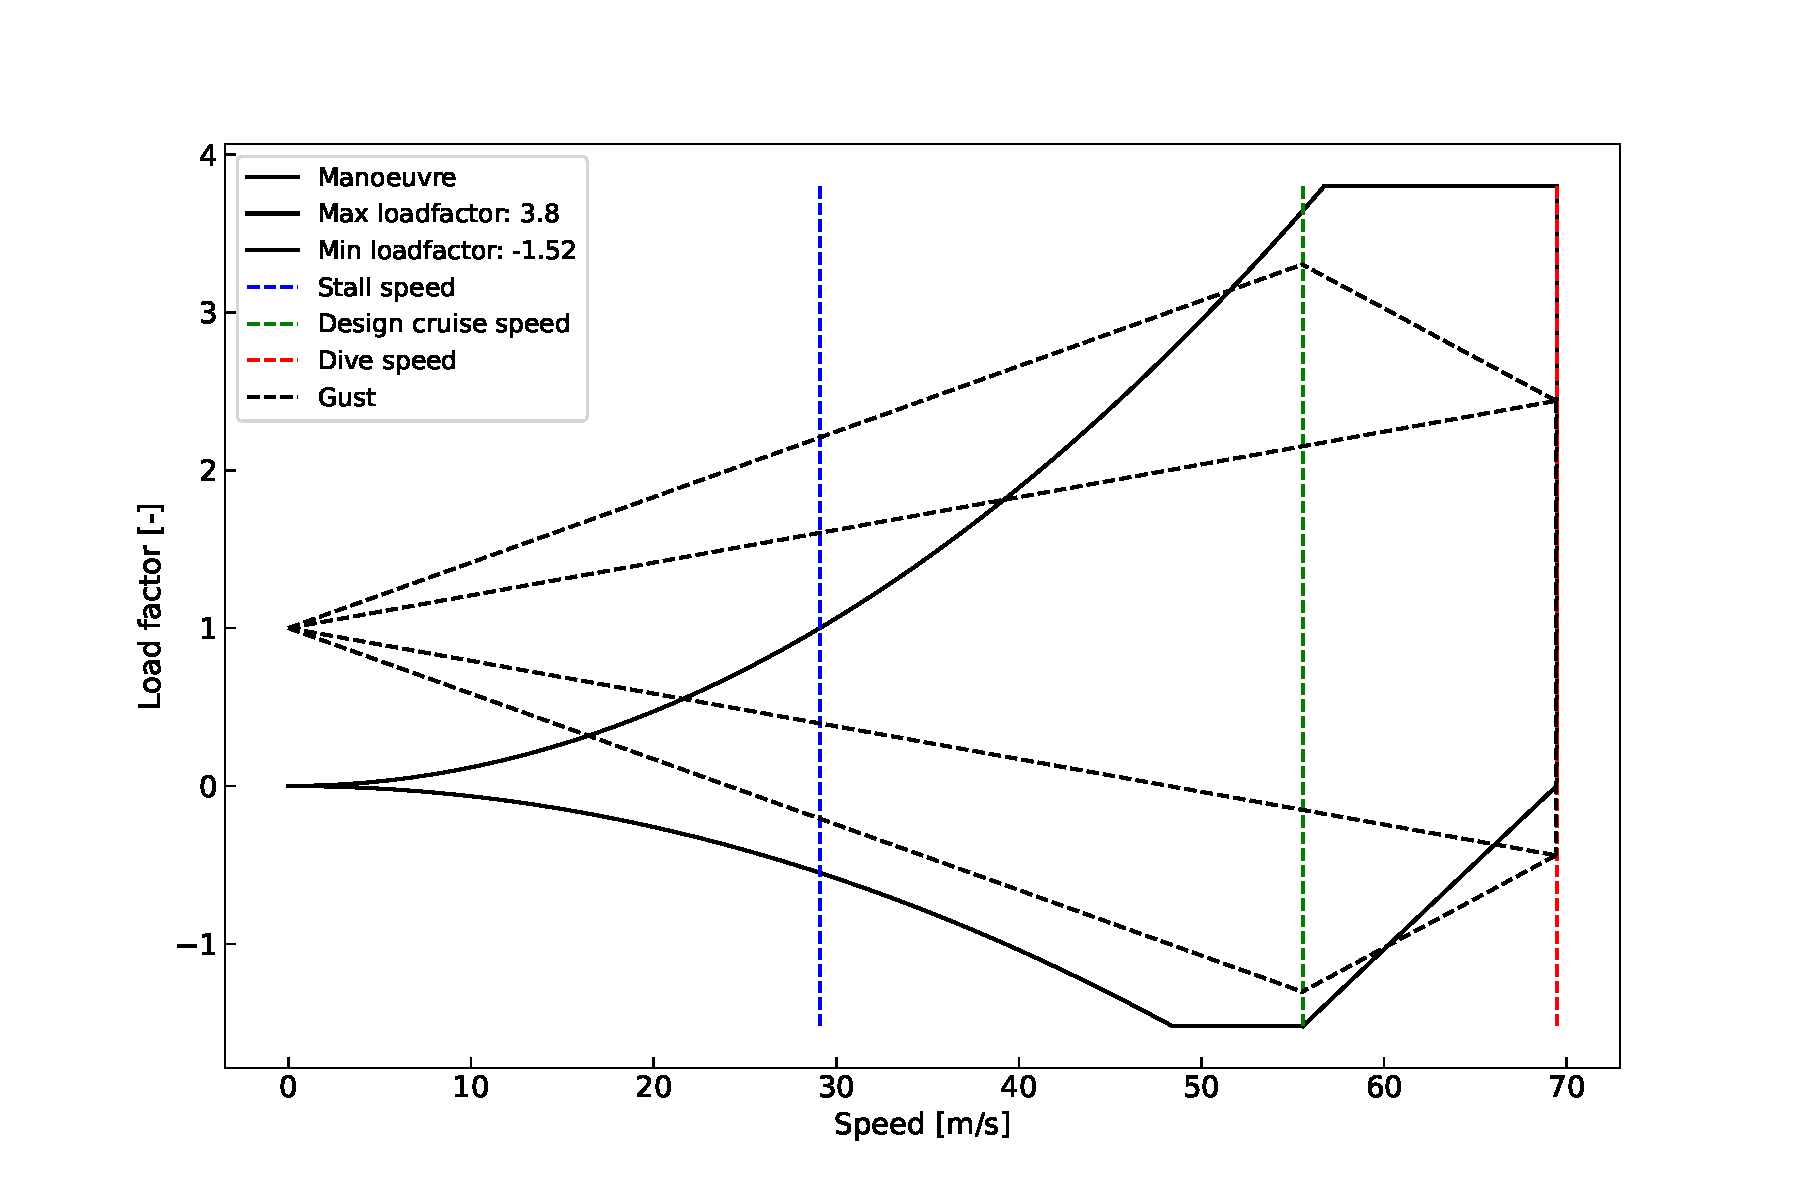
\includegraphics[width=0.8\linewidth]{figures/Structures/VN_diagram}
    \caption{Final load diagram}
    \label{fig:struc:Load_diagram}
\end{figure}

\section{Wing Structural Design}
In order to design the structure of the wing, it is essential to first identify what the critical load cases are.
For this scope, both configurations, cruise and take-off, are analysed.
Spars, ribs, and skin are then sized accordingly.
A separate discussion is then carried out with regard to the hinge design and mechanism.

\subsection{Load Cases}
\label{sec:loads}
In order to calculate what each section of the structure needs to be able to withstand, all loads acting on the wing need to be accounted for.
These are shown in \Cref{fig:LoadConfig} for cruise and take-off configurations.
The distributed loads of lift ($L$) and wing weight ($W_\text{wing}$) are assumed to be elliptical and trapezoidal respectively.
Point forces are then introduced by the engine weight ($W_\text{eng}$) and thrust ($T_\text{eng}$).
Several considerations need to be made to construct the shear force, bending moment, and torque diagrams.
Firstly, the aerodynamic centre and the CG at each section of the wing are assumed to be at 0.25 and 0.4 of the chord length.
Secondly, the engine’s longitudinal CG is also considered at 25\% of the chord.
This can be easily reached by slight adjustments in position, nacelles, and component distribution.
These displacements of aerodynamic forces and engine weight compared to the CG of the section are the main contributors to the twist of the wing.
Thirdly, the battery weights ($W_\text{bat}$) are assumed to be equally distributed in the two outer nacelles.
The resulting diagrams are shown in \Cref{fig:LoadingDiagramsCruise,fig:LoadingDiagramsTO}.

%\begin{figure}[h]
%    \centering
%    \includegraphics[width=\linewidth]%{figures/LoadingConfigurationCruise}
%    \caption{All forces and moments acting on the wing in cruise %configuration}
%    \label{fig:LoadConfigCruise}
%\end{figure}

%\begin{figure}[h]
%    \centering
%    %\hspace{2.5cm}
%    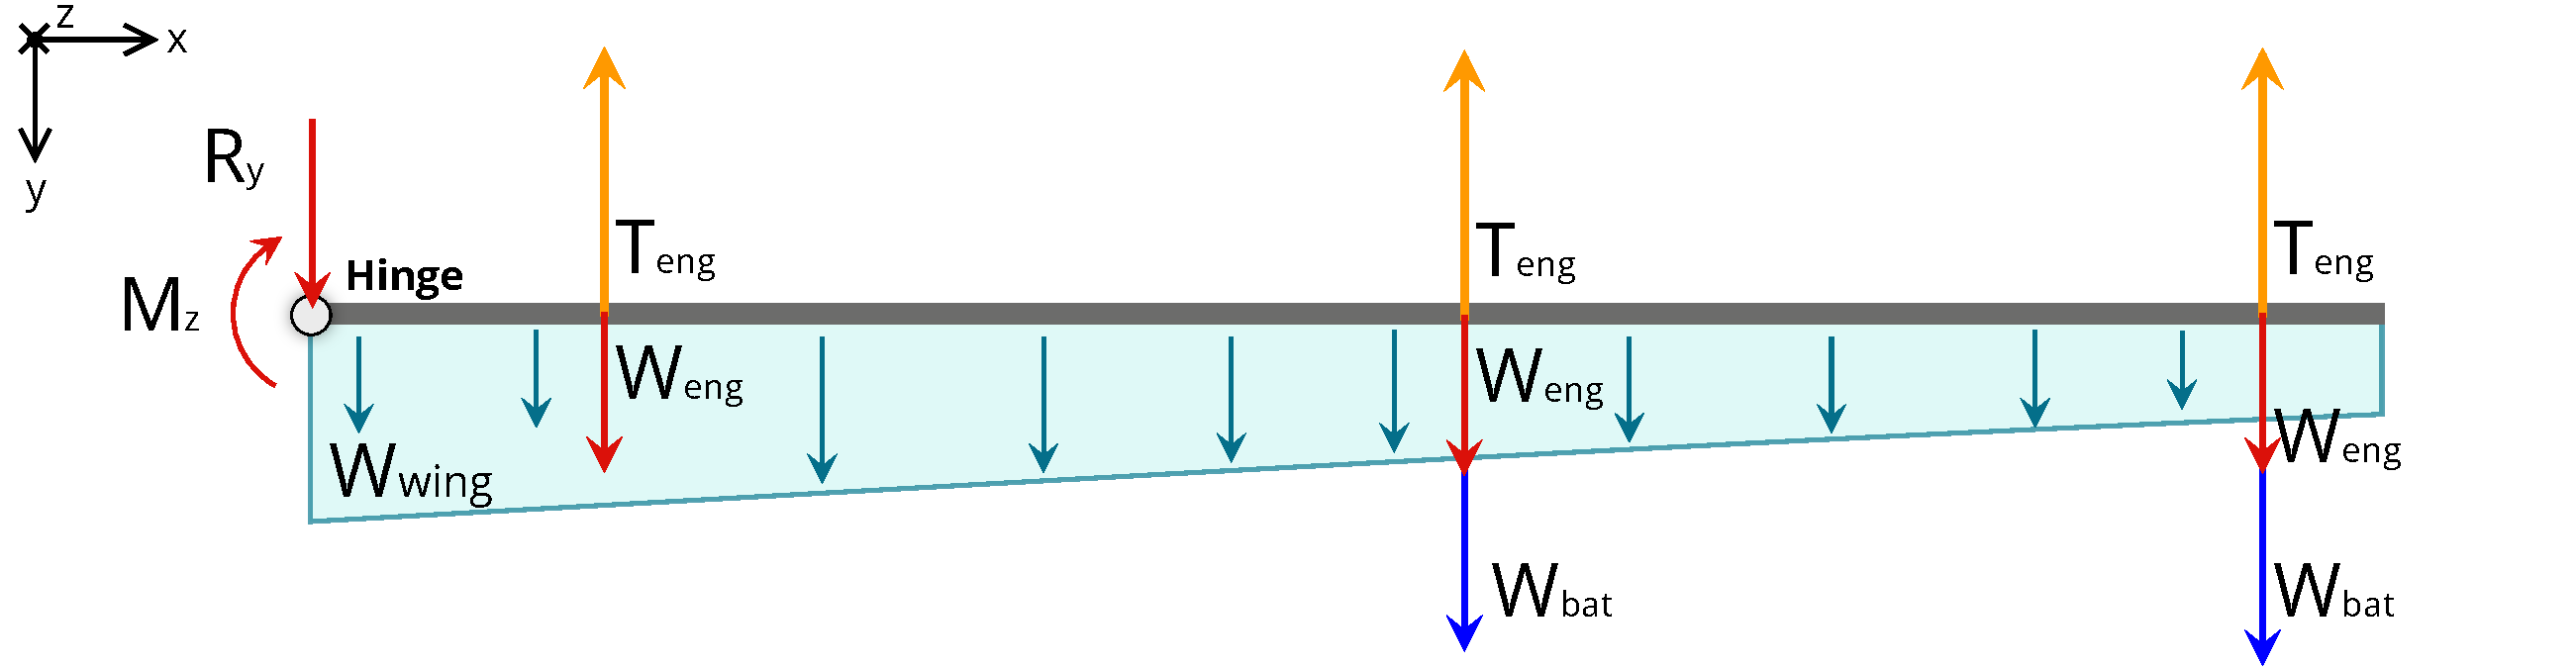
\includegraphics[width=1\linewidth]{figures/LoadingConfigurationTO2}
%    \caption{All forces and moments acting on the moving part of the wing during take-off}
%    \label{fig:LoadConfigTakeoff}
%\end{figure}

\begin{figure}[H]
    \centering
    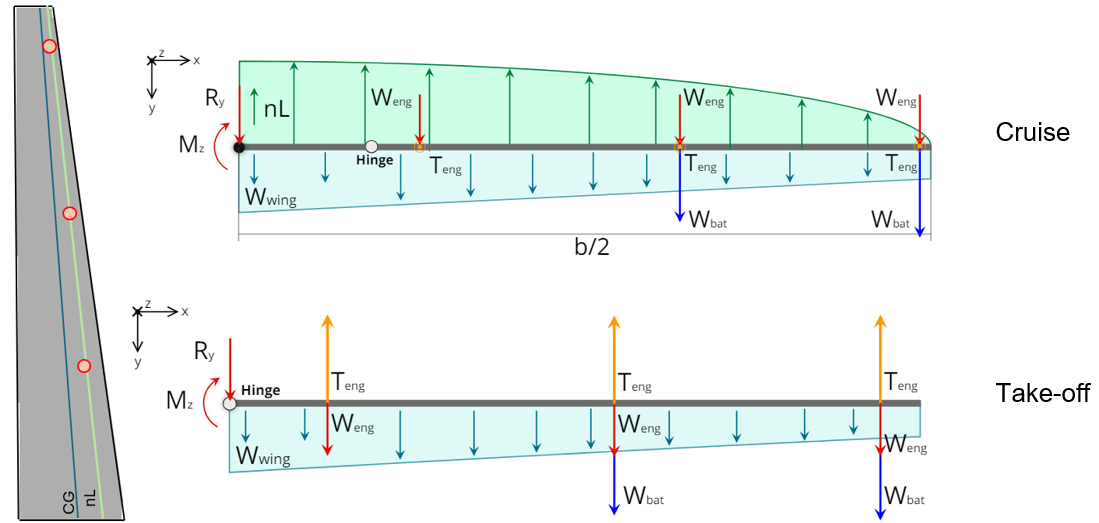
\includegraphics[width=1\linewidth]{figures//Structures/LoadingWing.png}
    \caption{All forces and moments acting on the wing in cruise and take-off configurations. The top view (left) shows the location of the resultant aerodynamic forces and the cg of the engines (red dots) with respect to the chord.}
    \label{fig:LoadConfig}
\end{figure}

\begin{figure}[H]
    \centering
    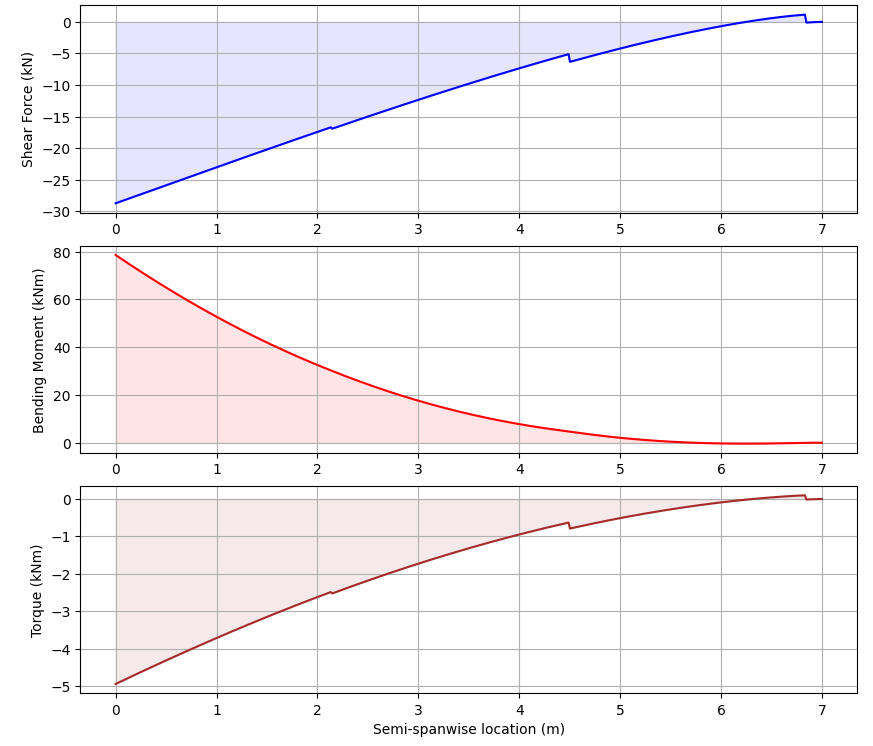
\includegraphics[width=1\textwidth]{figures/Structures/LoadCruise.png}
    \caption{Shear force, bending moment, and torque diagrams in cruise, n = 4.1}
    \label{fig:LoadingDiagramsCruise}
\end{figure}

\begin{figure}[h]
    \centering
    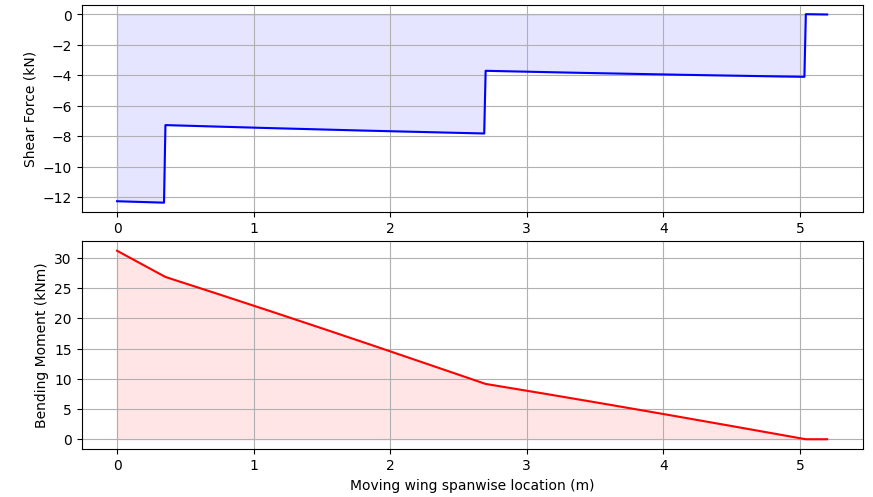
\includegraphics[width=\textwidth]{figures/Structures/LoadTO.png}
    \caption{Shear force and bending moment diagrams in take-off, T/W = 2}
    \label{fig:LoadingDiagramsTO}
\end{figure}

It can be noticed how the wing span considered in the two scenarios is different.
This is because in \Cref{fig:LoadingDiagramsTO} only the diagram concerning the moving part of the wing is shown.
The most critical loads are identified to be as follows:
\begin{itemize}
    \item 29 kN shear force at the root of the wing during cruise;
    \item 80 kNm of bending at the root of the wing during cruise;
    \item 32 kNm of torque on the fixed part of the wing during take-off.
\end{itemize}
These loads will prevail in the sizing of the central wing box, while a different discussion is carried out with regard to the hinge in \Cref{sec:hingedesign}.
In order to simplify the analysis and sizing of the wing structure, conservative assumptions are made on the carrying capabilities of each component.
The bending moments are assumed to be taken by the spars and the stringers.
Ribs, instead, introduce local loads into the structure, transfer aerodynamic loads from the skin to the structure, and prevent buckling.
A rectangular torsion box is finally analysed to ensure the spars, together with the stiffened skin panels, can withstand the induced torques.
It is important to note that the integration of all of these components together is not an easy exercise, and the ribs-stiffeners interactions need particular attention to ensure the load paths are not disturbed.
Finally, a safety factor of 1.5 is used for all dimensions to overcome uncertainties in the calculations as well as guarantee safety during most unexpected scenarios.

\subsection{Wing Spars}
\label{sec:wingspar}
Two spars are placed in the wing, each one at the edges of the wingbox and located at 25\% and 75\% of the chord, respectively.
For sizing, however, most bending moments are assumed to be taken by the front spar and the stiffeners.
This assumption is conservative and adds to the safety factor already considered.
A variable thickness with a linear distribution is considered throughout the span to ensure minimum weight while still allowing for changing loads.
A fixed thickness, however, is used in the fixed part of the wing, where the main torsion box is placed.
This is done to ensure the robustness of the structure.
The spars are made of aluminium 7040-T7451 as selected in \Cref{sec:matselection}, and its mechanical properties, assuming linearly elastic behaviours, apply to the calculations.
Furthermore, the interruption of the spars due to the cut in the folding wing is neglected in the analysis.
This is because the hinge design and its locking mechanisms are considered able to create load paths that well reproduce those of a standard wing.
Last but not least, a symmetric wingbox is assumed ($I_{xy} = 0$) such that the stresses caused by the bending moments are calculated as follows:

\begin{equation}
    \sigma_z = \frac{M_xI_{yy}y + M_xI_{xx}x}{I_{xx}I_{yy}}
    \label{eq:normalstress}
\end{equation}
Here, the $M$'s refer to the bending moments in different directions, the $I$'s refer to the area moments of inertia, and $x$ and $y$ correspond to the respective coordinates within the cross-section.
As the area moments of inertia are greatly dependent on the shape of the cross-section, a standard I-beam spar design is chosen.
By taking into consideration both cruise and take-off conditions, the optimal spar design for minimal weight is found.

The spars, however, constitute the side walls of the wingbox, which also take care of counteracting the torque.
The shear flow caused by the shear forces (\Cref{eq:shear}) as well as the torques (\Cref{eq:torque}) acting on the wing is thus considered, and their effect is summed up.


\begin{equation}
    q_2 - q_1 = -\frac{V_y}{I_{xx}}\int_{s_1}^{s_2}ty \ ds -\frac{V_x}{I_{yy}}\int_{s_1}^{s_2}tx \ ds
    \label{eq:shear}
\end{equation}


\begin{equation}
     t_{\min} = \frac{1}{\tau_{\text{shear}_{\max}}} \frac{T}{2 \cdot A_\text{enclosed}}
    \label{eq:torque}
\end{equation}


In these equations, $q$ indicates shear flow, $V$ refers to the shear forces as calculated previously, and $A_\text{enclosed}$ is the area enclosed by the cross-section of the wing box.
The integrals are computed across the entire perimeter.
The spar thickness is thus calculated again and compared to the one needed to withstand the bending moments.
The maximum value is chosen and used in the wing.
Some reference values are shown in \Cref{tab:wingstructure}.


\subsection{Wing Ribs}
\label{sec:wingribs}
As explained by Sedaghati et al. \cite{sedaghati2006wing}, the ribs are responsible for three kinds of loads:
aerodynamic loads introduced from the skin-stiffeners panel,
point loads on the wing, and body forces, like the weight of the wing.
Furthermore, while running from the leading to the trailing edge of the wing, the ribs are divided into three sections, in between which spars are accommodated.

For the positioning of the ribs, it is thus chosen to place them where the engines are placed, at the edges of the ailerons, and close to the hinge.
Furthermore, as the distance between the ribs may influence the buckling performance of the skin, this is later checked to be sufficient.
Following this reasoning, the ribs have been placed at the x locations indicated in \Cref{tab:wingstructure}, starting from the root.
As far as their dimensions are concerned, similar dimensions to the spars placed at different locations are used.


\subsection{Stiffeners-Reinforced Skin Panel}
As the biggest wing deflections are expected in the upward direction during cruise flight, buckling of the upper skin panel is considered critical. 
The critical stress for buckling of a panel can be calculated using \Cref{eq:buckling}.

\begin{equation}
\label{eq:buckling}
    \sigma_{cr} = C \frac{\pi^2E}{12(1-\upsilon^2)} \left(\frac{t}{b}\right)^2
\end{equation}


Where $E$ is the Young’s modulus, $\upsilon$ is the Poisson ratio, $t$ the thickness of the plate, and $b$ is the panel span in the load’s direction.
Finally, $C$ is a function of the aspect ratio and boundary conditions of the plate.
Here, a $C$ of 4.0 with the conservative assumption of the skin panel being simply supported on all sides is considered.
Taking into account that the skin is supported by stiffeners, their crippling stress needs to be calculated.
This is done by slightly modifying \Cref{eq:buckling}:

\begin{equation}
\label{eq:crippling}
    \frac{\sigma_{cc}}{\sigma_y} = \alpha \left[\frac{C}{\sigma_y} \frac{\pi^2E}{12(1-\upsilon^2)} \left( \frac{t}{b} \right)^2\right]^{1-n}
\end{equation}

where $\sigma_{cc}$ and $\sigma_y$ are the crippling and yield stress of the material, $\alpha = 0.8$, and $n = 0.6$. This calculation is applied to each panel forming the stiffener and using appropriate boundary conditions.
A weighted average with the areas is then performed to find the crippling stress of the entire stiffening element.
By use of \Cref{eq:We}, the influence of the stringer on the panel is calculated, and the buckling stress of the stiffened panel is finally obtained.


\begin{equation}
\label{eq:We}
    w_e = \frac{t}{2} \sqrt{ \frac{C \pi^2}{12(1-\upsilon^2)} \frac{E}{(\sigma_{cc})_\text{stiffener}}}
\end{equation}

In the case of a reinforced skin panel, the cross-section of the stiffening elements influences the assumptions on the panel boundary conditions, as this can greatly influence the torsional stiffness.
For this reason, Hat types are considered for stringers, resulting in a $C = 6.98$~\cite{curtis1997fundamentals}.
The value of C, in reality, is also based on the spanwise length of the panel, thus revealing the dependence of the buckling capabilities of the skin on the ribs positioning.
The rib spacing is used here, as found in \Cref{sec:wingribs}
An iterative process to minimise the mass has been adopted.

As it was done for the spars, the skin is subjected to the shear flow due to torque and shear.
The same procedure as in \Cref{sec:wingspar} is adopted, and the highest value for the skin thickness is chosen.
The results obtained are shown in
\Cref{tab:wingstructure}.


\subsection{Final Wing Structure Parameters}
\Cref{fig:WingDrawing} shows one section of the wing and the internal wing box structure.
The parameters considered for the design are indicated here.
Their final values for each of the wing sections are in \Cref{tab:wingstructure}.

\begin{figure}[!htb]
    \centering
    \begin{minipage}{.8\textwidth}
        \centering
        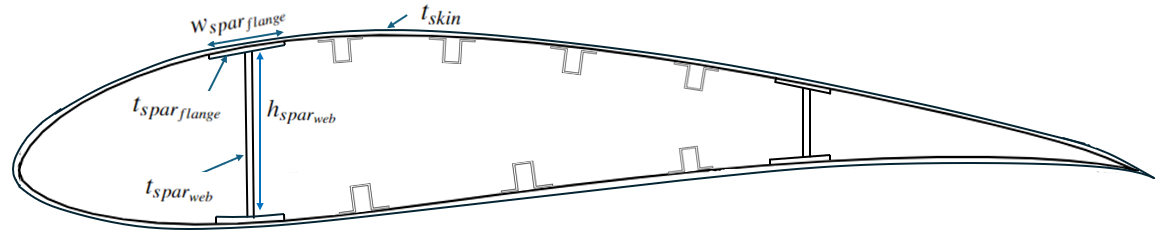
\includegraphics[width=\linewidth]{figures//Structures/WingBoxStructure.png}
        \caption{Wing section showing the internal wing box structure}
        \label{fig:WingDrawing}
    \end{minipage}%
    \begin{minipage}{0.2\textwidth}
        \centering
        \centering
        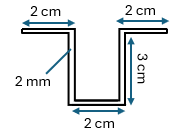
\includegraphics[width=1.0\linewidth]{figures//Structures/HatStiffener.png}
        \caption{Hat stiffeners dimensions}
        \label{fig:hatstiffener}
    \end{minipage}
\end{figure}



% Please add the following required packages to your document preamble:
% \usepackage[table,xcdraw]{xcolor}
% Beamer presentation requires \usepackage{colortbl} instead of \usepackage[table,xcdraw]{xcolor}
\begin{table}[H]
    \centering
    \caption{Transposed wing structure parameters, with $x$ [\unit{m}] as the distance from the root}
    \label{tab:wingstructure}
    \sisetup{table-auto-round}
    \resizebox{\textwidth}{!}{
    \begin{tabular}{
        S[table-format=1.2]
        |S[table-format=3]
        S[table-format=1.2]
        S[table-format=2]
        S[table-format=1.1]
        S[table-format=1.1]
        S[table-format=1]
        S[table-format=1]
    }
        \toprule
        \textbf{$x$ {[}\unit{m}{]}} & \textbf{$h_{\text{spar}_\text{web}}$ {[}\unit{mm}{]}} & \textbf{$t_{\text{spar}_\text{web}}$ {[}\unit{mm}{]}} & \textbf{$w_{\text{spar}_\text{flange}}$ {[}\unit{mm}{]}} & \textbf{$t_{\text{spar}_\text{flange}}$ {[}\unit{mm}{]}} & \textbf{$t_\text{skin}$ {[}\unit{mm}{]}} & \textbf{$N_{\text{stringers}_\text{top}}$ [\unit{-}]} & \textbf{$N_{\text{stringers}_\text{bottom}}$  [\unit{-}]} \\ \midrule
        0 & 227 & 1.5 & 50 & 2.8 & 1.5 & 4 & 3 \\
        0.85 & 211 & 1.5 & 50 & 2.8 & 1.5 & 4 & 3 \\
        1.8 & 192 & 1.34 & 50 & 2.5 & 1 & 4 & 3 \\
        2.15 & 185 & 1.31 & 50 & 2.5 & 1 & 4 & 2 \\
        4.5 & 140 & 1.11 & 50 & 2.5 & 1 & 3 & 2 \\
        6.84 & 94 & 0.91 & 50 & 2.5 & 1 & 2 & 1 \\ \bottomrule
    \end{tabular}
    }
\end{table}

Inspection of \Cref{tab:wingstructure} can help get a better overview of what the final wing structure design looks like.
It is important to highlight how the number of stringers for each wing section was chosen based on meeting buckling and bending moment requirements.
Buckling was, in fact, found to be critical in the fixed part of the wing, while bending required a higher number of stiffeners in the outer part.
Furthermore, the different numbers of stringers on the top and bottom skin are due to the lower absolute value in the minimum load factor.

\section{Aeroelastic Analysis}
To achieve aeroelastic certification in accordance with CS23 requirements, the aircraft must exhibit no signs of aeroelastic effects across airspeeds ranging from 0 to 1.15V\(_D\) at all operational altitudes \cite{easa2018easy}. Several aeroelastic effects need to be evaluated, including wing divergence, control reversal, and flutter. While a comprehensive aeroelastic analysis is recommended for the future, the current focus is solely on wing divergence.

Wing divergence is a critical aeroelastic phenomenon where the aerodynamic forces acting on a wing structure become sufficiently strong to cause static instability. This leads to a dramatic and often catastrophic deformation of the wing.  Understanding and predicting the divergence speed at which this instability occurs is essential for the safe design of aircraft wings. The divergence boundary represents the critical dynamic pressure threshold that distinguishes between conditions where an aircraft experiences divergence and where it does not. This boundary is called such because the airspeed corresponding to this dynamic pressure changes with altitude. As a result, when the divergence speed is plotted against altitude, a boundary curve is formed. Beyond this speed, the twist angle of the wing increases without bound in response to a perturbation. \Cref{eq:divergence} is used to calculate the divergence dynamic pressure. A detailed derivation can be found in the \enquote*{AE4ASM506 Fundamentals of Aeroelasticity} lecture notes.


\begin{equation}
    q_\text{div} = \frac{K_\theta}{C_{L_\alpha}eS}
    \label{eq:divergence}
\end{equation}

In \Cref{eq:divergence} $q_\text{div}$ represents the divergence boundary in [N/m$^2$], $K_\theta$ the torsional stiffness of
the section in [Nm/rad], $C_{L_\alpha}$ the lift curve slope of the airfoil in [1/rad], $S$ the wing
surface area per unit span of the total aircraft in [\unit{m^2}], and $e$ the distance between the aerodynamic centre and the elasticity axis [m]. The latter is considered to be at the centre of the wingbox as a consequence of its previously assumed symmetry. The section at the MAC is taken into consideration for the analysis. It is thus assumed that this section of the aircraft wing exhibits a similar aeroelastic response to that of the full 3D wing. When this section is aeroelastically stable, the full 3D wing will be also stable. Assuming that the elasticity axis is located at the centre of the wingbox, and with a calculated $K_\theta$ of 144.9 kNm/rad, \Cref{eq:divergence} yields a $q_\text{div}$ = \qty{91.6}{kN/m^2}, corresponding to a sea level speed of 1392.5 km/h. A wing divergence speed of 1400 km/h is quite high and would typically be associated with high-performance aircraft, such as military jets or high-speed experimental aircraft. This high divergence speed indicates a very stiff and strong wing structure, capable of withstanding significant aerodynamic forces without experiencing divergence. 

\section{Hinge \& Folding Mechanism Design}
\label{sec:hingedesign}
The finished detailed wing structure design allows the sizing of the hinge and folding mechanism enabling the ground footprint of the UAM. In the following section, the steps taken to realise the design of this subsystem are presented.
Firstly, the design of the degrees of freedom is performed by building a kinematic simulation.
Subsequently, the hinge is sized for the identified maximum load case.
Ultimately, the actuation system is selected which can counteract the torques during the transition.

\subsection{Hinge Axis of Rotation}
\label{subsec:axis}
\label{sec:hinge_axis_of_rotation}
The design of the hinge, facilitating the transition of the vehicle, starts with the appropriate selection of the degrees of freedom and rotational axes.
From previous aircraft designs, it was found that such wing transformations can be done about only one rotational axis \cite{pterodynamics_site}.
Thus, it is opted to select a joint design with only one rotational degree of freedom, since this decision decreases the complexity of the design and consequently increases the safety of the vehicle operations.


To aid the selection of the rotational axis, it was parameterised with the angles $\alpha$ and $\beta$ as depicted on \Cref{fig:angle_axis_rotation}.
Furthermore, the unit vector \textbf{n} parallel to this axis is given by \Cref{eq:angle_axis_rotation}.
Finally, the rotation matrix about a unit vector $n$ by a rotation angle $q$ is given by \Cref{eq:angle_axis_rotation}, where the skew-symmetric matrix, $n_{\times}$, is constructed from the vector $n$.
Utilizing this equation, the full range of rotational motion can be simulated for a given rotational axis.
To facilitate a better understanding of this one degree of freedom motion, a visual kinematic simulation of the motion was developed in Python.
Two frames of this simulation can be seen in \Cref{fig:angle_axis_rotation,fig:rot_sim}. This tool could then be used to select the optimal values of the parameters.
It is desired that the wing is horizontal and almost vertical, with a slight tilt towards the outside, in the body frame at the start and the end of the transition respectively.
Thus, after running the simulations for different parameters, it was found that an $\alpha$-value of \qty{45}{\deg}, a $\beta$-value of \qty{40}{\deg} and a rotation angle range of $q \in [\qty{0}{\deg}; \qty{110}{\deg}] $ results in a satisfactory range of motion.
\begin{align}
\label{eq:angle_axis_rotation}
    \textbf{C}_n(q) &= \cos(q)\textbf{I}_{3\times 3} + \sin(q) \textbf{n}_{\times} + (1-\cos(q))\textbf{n}\textbf{n}^T & & \textbf{n} =\frac{\begin{bmatrix} \cos(\alpha) & \sin(\alpha) & \sin(\beta) \end{bmatrix}^T}{\sqrt{\cos(\alpha)^2+\sin(\alpha)^2+ \sin(\beta)^2}}
\end{align}

\begin{figure}[!htb]
    \centering
    \begin{minipage}{.5\textwidth}
        \centering
        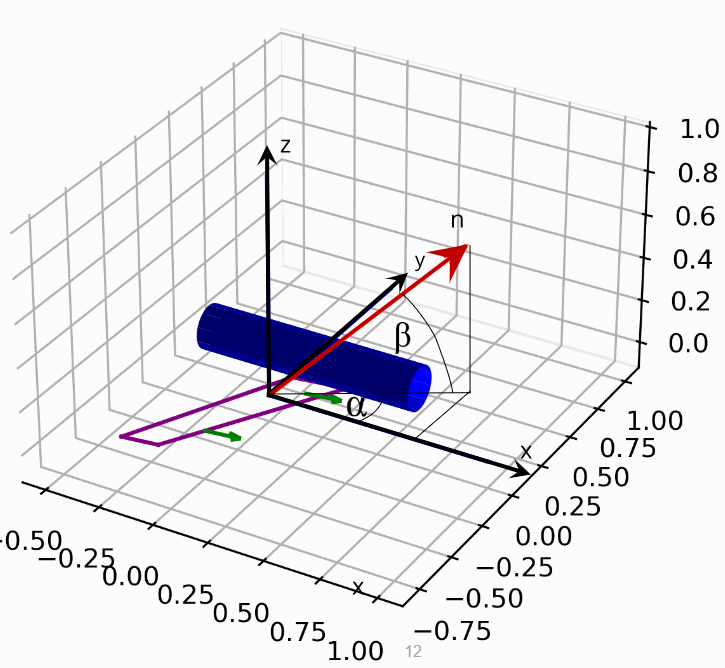
\includegraphics[width=0.95\linewidth]{figures/Structures/rot_sim_2.png}
        \caption{Snapshot of the kinematic wing rotation simulation, midway through transition}
        \label{fig:angle_axis_rotation}
    \end{minipage}%
    \begin{minipage}{0.5\textwidth}
        \centering
        \centering
        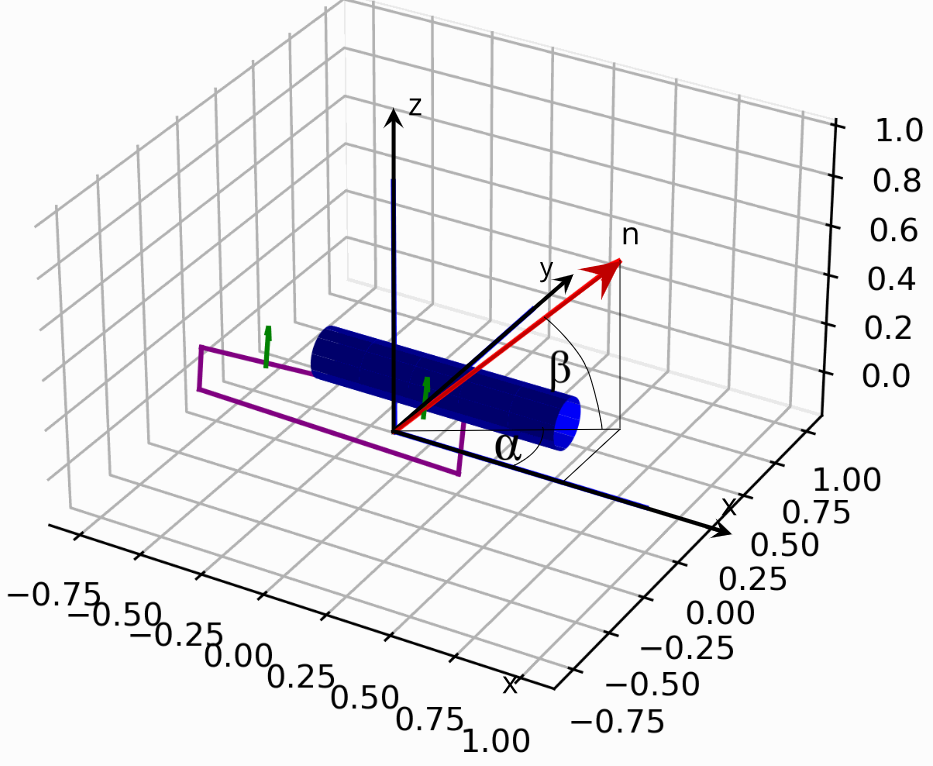
\includegraphics[width=1.0\linewidth]{figures/Structures/rot_sim.png}
        \caption{Snapshot of the kinematic wing rotation simulation, hexacopter configuration}
        \label{fig:rot_sim}
    \end{minipage}
\end{figure}

\subsection{Hinge Sizing}

As the hinge allowing the transition between take-off and cruise configuration is considered critical for the design, a thorough analysis of the loads that this needs to withstand is performed and the hinge is sized accordingly.
The axis of rotation identified in \Cref{subsec:axis} is used to choose the type of hinge.
For ease of certification, as well as a reduction in design and production costs, it is opted for the adaptation of a pre-existing hinge mechanism.
In particular, the STO Wing folding mechanism used by the Grumman F4F-4 Wildcat was found to be of particular interest (\Cref{fig:WildcatHinge}).

\begin{figure}[H]
    \centering
    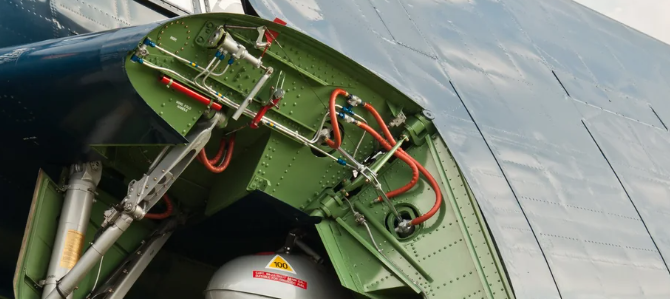
\includegraphics[width=0.65\linewidth]{figures//Structures/GrummanWildcatHinge}
    \caption{Grumman F4F-4 Wildcat STO wing folding mechanism}
    \label{fig:WildcatHinge}
\end{figure}

For the structural analysis, the hinge is modelled as a rod-lug mechanism with the rod in the direction of the axis of rotation.
Loads at the hinge location are taken from \Cref{sec:loads} and a coordinate system transformation is performed as shown in \Cref{fig:coordtransf} in order to decompose the forces and moments in the rod-lug directions.
The stresses are then considered.
Stainless steel, Al 7075-T6 and titanium were used for the analysis.
Taking into account cost factors and weight, titanium was chosen as the hinge material with a density of \qty{4500}{kg/m^3} and a tensile ultimate strength of 220 MPa.

\Cref{tab:hingeforces} shows the results obtained in terms of forces and moments.
Although the moments in the $z$- and $y$-directions are perpendicular, meaning the maximum normal stresses they cause in the rod do not sum up, they are here superimposed and used in \Cref{eq:normalstress}.
This is a rather conservative assumption and counts as a safety factor.
Normal stresses caused by normal forces are also accounted for ($\sigma = N/A$). Performing these calculations for the rod yields a minimum radius of 7.8 cm.
This, together with a length of 25 cm based on the height of the wing and inclination of the hinge, yields an estimated mass of the hinge of 21.5 kg.

As Kothia et al. \cite{kothia2016design} have performed an adaptation of the same joint to a Boeing 787 with a comprehensive 
study of sizing via Finite Element Method (FEM) analysis and their results are used for validation.
A linear scaling of the weight of the aircraft leads to a hinge weight of $\approx$ 18 kg each.
This is not too far off the 21.5kg calculated, which did indeed take several conservative assumptions into account.

\begin{minipage}{.5\textwidth}
\begin{figure}[H]
    \centering
    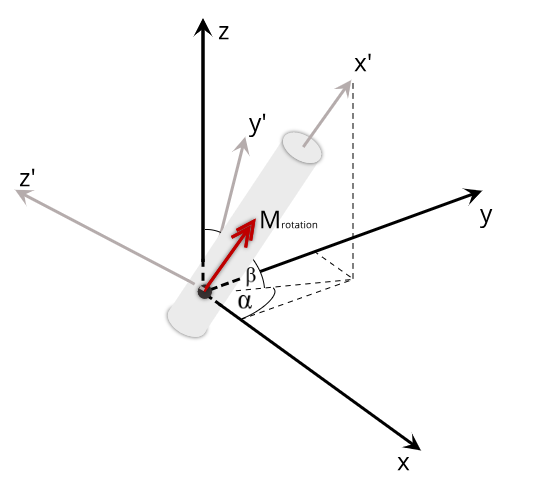
\includegraphics[width=0.7\linewidth]{figures/Structures/force_decomp}
    \caption{Coordinate transformation to decompose forces in the direction of the hinge.}
    \label{fig:coordtransf}
  \end{figure}
\end{minipage}
\begin{minipage}{.5\textwidth}
\begin{table}[H]
    \centering
    \caption{Maximum loads experienced by the hinge. Note that all occur during cruise with $n=4.1$}
    \begin{tabular}{lS[table-format=+2.1]l}
        \toprule
        \textbf{Load Type} & \multicolumn{2}{c}{\textbf{Magnitude}} \\ \midrule
        Normal force ($x$) & 18.4 & kN\\
        Moment in $y$ & 43.4 & kNm \\
        Moment in $z$ & -36.5 & kNm\\ \bottomrule
    \end{tabular}
    \label{tab:hingeforces}
\end{table}
\end{minipage}
 

In the previous calculations, the entirety of the loads were assumed to act on the hinge itself.
However, locking mechanisms and load-carrying structures are to be placed at the cut of the wing.
Specifically, locking arms are expected to extend out from the moving wing to its fixed part, connecting the two and also preventing discontinuities in the wing twist caused by aerodynamic forces.
These ensure a more homogeneous transfer of the loads between the two parts of the wing, as well as help relieve the loads on the hinge.

\subsection{Actuator Choice \& Power }

Once the hinge has been designed, its actuator system needs to be implemented.
The power used for the folding and unfolding of the wing is first estimated by looking at the moments acting in the direction of the axis of rotation, as decomposed in \Cref{fig:coordtransf}.
Assuming transition can be initiated during cruise conditions (with $n = 1$) or during take-off, the latter was found to be constrained in terms of power required, with a moment of $\approx$ 15 kNm to be provided to the hinge.
The power is then estimated assuming a constant angular velocity around the axis during transition.
With a rotation of \qty{110}{\deg} needed and 63 seconds used to transition (see \Cref{subsec:transition}), this comes down to an angular speed of $\omega = 0.0305$ rad/s.
The power required is finally estimated with $P_r = \omega \cdot M_\text{rotation} = 458$ W. This value is added to the power budget computed in \Cref{ch:Resource_Allocation_and_Budget_Breakdown}.
Note, however, that especially during the unfolding of the wing, the thrust of the engines is expected to reduce the power needed from the actuator.

Linear actuators which would pull and push the trailing edge of the wing were considered.
However, it is ultimately opted for actuators located within the wing structure.
Having the booms of the actuator running between the wing and fuselage on the outside of the aircraft was, in fact, found not to be ideal in terms of aerodynamics and reliability.
Two main types are thus considered:
\begin{itemize}
    \item \textbf{Rotary gears} (\Cref{fig:rotarygears}): a motor can be disposed within the rotating wing portion to rotate a drive gear that can be meshed with a stationary gear rack placed on the fixed wing portion.
        This would result in the drive gear travelling around the circumference of the other rack.
    \item \textbf{Opposed linear actuators} (\Cref{fig:linearactuators}): these can be hydraulic, electric, or pneumatic linear actuators and would allow the rotation of the joint by extension of the arms.
\end{itemize}

\begin{minipage}{0.5\linewidth}
    \begin{figure}[H]
    \centering
    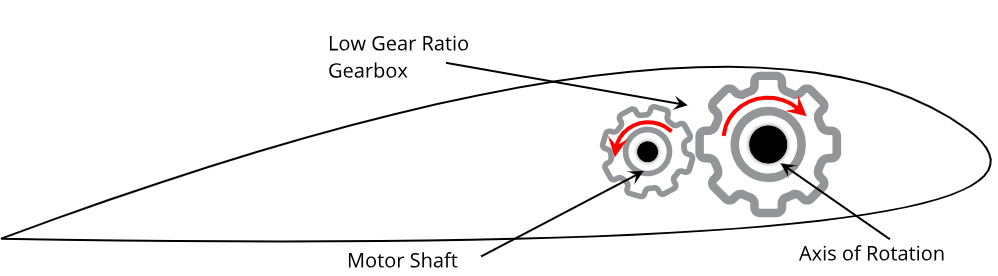
\includegraphics[width=1\linewidth]{figures/Structures/gearbox_actuator}
    \caption{Rotary gears schematics.}
    \label{fig:rotarygears}
    \end{figure}
\end{minipage}
\begin{minipage}{0.5\linewidth}
    \begin{figure}[H]
    \centering
    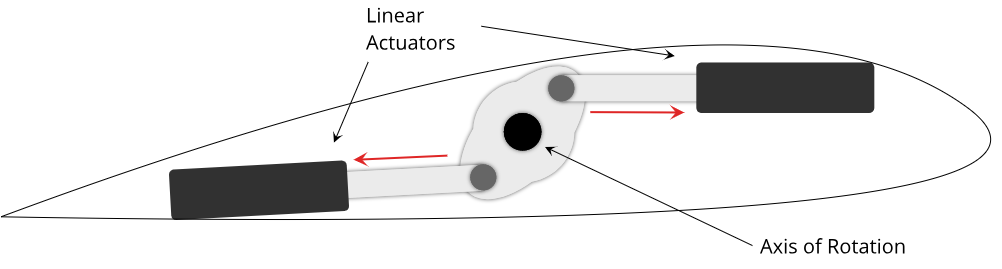
\includegraphics[width=1\linewidth]{figures/Structures/pneumatic__actuator}
    \caption{Linear actuators schematics.}
    \label{fig:linearactuators}
    \end{figure}
\end{minipage}

For rotary gear actuators, a low-ratio gearbox with a high-torque motor would be needed to counteract the moments experienced by the wing during transition.
Such actuators are relatively large, thus, the integration of it into a slender wing would be challenging.
Furthermore, high power is required to operate the high-torque motor.
Hence, the application of such an actuator is not favourable.

Ultimately, it was thus chosen to use the linear actuators shown in \Cref{fig:linearactuators}.
The little arm between the actuators and the axis of rotation would allow for smaller forces to be applied.
Furthermore, failure of one of the actuators would not hinder the folding capabilities of the wing, with each of the actuators designed to provide enough torque alone, despite resulting in a smaller angular velocity. \Cref{fig:hingeinwing} shows the positioning of the actuators in the wing as presented by Pterodynamics \cite{PteroPatent}. The entire wing structure is modified around the cut to accommodate the presence of the actuator and to allow proper redistribution of forces and moments.

\begin{figure}[H]
    \centering
    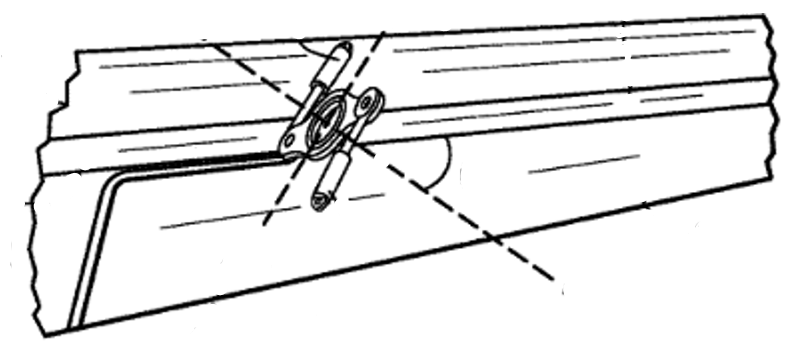
\includegraphics[width=0.5\linewidth]{figures//Structures/ActuatorInWing.png}
    \caption{Integration of the linear actuator in the wing structure. The dashed line indicates the top view projection of the axis of rotation and its perpendicular \cite{PteroPatent}}
    \label{fig:hingeinwing}
\end{figure}

Amongst the different kinds of linear actuators, a choice has to be made. Electric actuators are chosen based on their excellent precision and control, with the ability to achieve precise positioning. Furthermore, they can easily be integrated with the computer control systems and automation setups. High efficiency with minimal energy losses is also guaranteed. Hydraulic actuators are excluded due to their higher weight (water is present), their complexity, and the need for regular maintenance. Pneumatic actuators, instead, can lead to less precise control and positioning due to air compressibility. 

%given the hinge type, their precision, design, and production costs, a rotary actuator was chosen. 
%However, given the proven compatibility with the hinge chosen, it was opted to reproduce the same actuation system used by the Grumman F4F Wildcat. This would also reduce the design and production costs of the actuator. 


\section{Undercarriage Design}
There are different configurations for the design of the landing gear for an eVTOL. There are two main options.
The first option is to use a non-retractable landing gear, skid or wheels, however, this will induce a lot of drag during flight and increase the $c_{d_{0}}$ which is unwanted.
The other option is to use retractable landing gear, which will come at the cost of extra power and space needed in the fuselage.
An efficient solution for this is to use a small nosewheel, similar to Lilium Jet (7-seater) \cite{lilium_jet} and have the other main landing gears inside the downward V-tail.
The nosewheel is covered by a cover to minimise the drag induced.
This is similar to a tricycle landing gear with the difference that the distance between the main landing gear and CG will be relatively high.

The tricycle landing gear has a single nosewheel and two main landing wheels.
  However,  stability has to be accounted for in the configuration since the aircraft can tip over.
    The longitudinal location of the CG is set at \qty{3.68}{m}.
The nosewheel must be located in front of this, and the main landing wheels must be located behind, which will be the case since they are in the tail.
Moreover, it is not allowed to place rigid structural components underneath the passengers due to safety reasons.
Therefore,
the location of the nosewheel should be in front of the front seat~\cite{SaullloCastro} at a location of \qty{1.5}{m} from the nose.
The main landing gears will be located in the empennage and the distance $l_{m}$ will be \qty{3.5}{m}.

The $y$-location of the main landing gear is dependent on the tip-over angle, $\psi$, the distance between the nose and the main landing gear and the longitudinal centre-of-gravity, $l_{n}$ and $l_{m}$, and the vertical centre-of-gravity location, $z$ which is 1.15 m from the ground, as seen in \Cref{ch:Stability_and_Control}.
The final equation can be seen in \Cref{eq:ylmg}.
\begin{equation}
    \label{eq:ylmg}
    Y_\text{MLG} > \frac{l_{n}+l_{m}}{\sqrt{\frac{l_{n}^2 \tan^2\psi}{z^2}-1}}
\end{equation}
\Cref{eq:ylmg} states that the $y$-location should be greater than 2.419.
This is to ensure that the vehicle does not tip over with the assumption that the tip-over angle should be lower than \qty{55}{\deg}\cite{ADSEEIslides}.
The horizontal span of the V-tail is 3.9 m, so in the case of $Y_\text{MLG} = 3.9$ the vehicle is stable.

The height of the landing gear has to be minimised to adhere to the vertical height requirement of two meters.
The landing gear consists of an absorber or damper which absorbs most of the energy during a hard landing.
The absorber stroke length, $s$, is set to \qty{0.2}{m} \cite{ADSEEIslides}.
The final values are put in \Cref{tab:undercarriage_values}.
\begin{table}[H]
    \centering
    \caption{Undercarriage sizing}
    \label{tab:undercarriage_values}
    \begin{tabular}{>{$}l<{$}|S[table-format=2.2]>{\collectcell\unit}l<{\endcollectcell}}
        \toprule
        \psi                  & 55                &  degrees                         \\
        l_{n}                 & 2.0                &  m          \\
        l_{m}                 & 3.5                 &  m           \\
        Y_\text{MLG} & 2.42& m \\
        z                       & 1.15                   &  m            \\
        s                       & 0.2              &  m         
                       \\\bottomrule
        
    \end{tabular}
    
\end{table}

\section{Verification \& Validation}
Verification and validation procedures are essential to ensure the accuracy of structural calculations in the code. To achieve this, the following steps are taken:
\begin{itemize}
    \item Repeated testing with known results: the code has undergone extensive testing by performing smaller exercises with known outcomes across different functions. 
    \item Optimization procedure verification: the optimisation process was rigorously checked by adjusting and varying each optimisation parameter individually. This controlled variation ensured that the optimisation parameters function correctly and sensibly within the intended range.
    \item Assumption verification: the equations used in the calculations often rely on certain underlying assumptions. Each of these assumptions is thoroughly checked to confirm their validity in the given context, ensuring that the equations are applicable and accurate for the specific scenario.
    \item Critical evaluation of results: the results were critically examined to ensure they are realistic and consistent with expected physical behaviour. This step helped identify any discrepancies or anomalies that could indicate errors in the calculations or underlying assumptions. 
\end{itemize}

By implementing these steps, the code’s robustness  and the reliability of the structural calculations it performs is ensured.


